% Load histograms for n=100000 balls (generated by figs_c2ch08.py, seed 8).
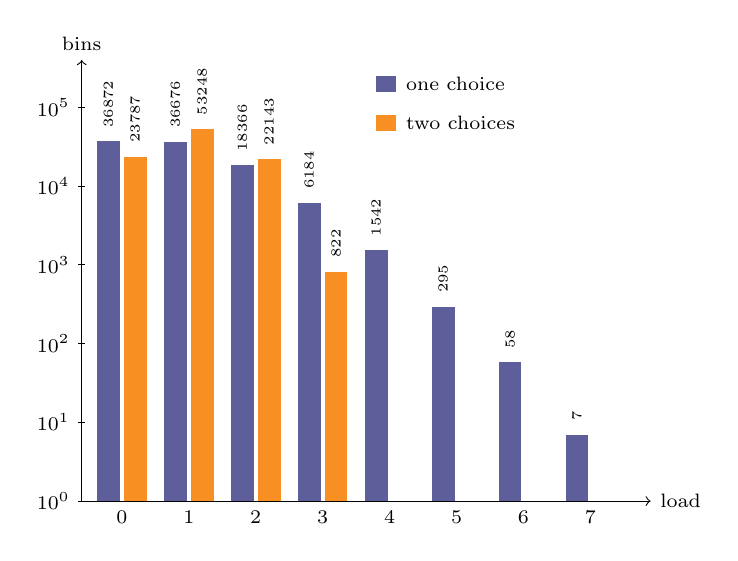
\begin{tikzpicture}[x=0.85cm,y=1cm,every node/.style={font=\scriptsize}]
\draw[->] (-0.6,0) -- (7.9,0) node[right] {load};
\draw[->] (-0.6,0) -- (-0.6,5.6) node[above] {bins};
\draw (-0.65,0) -- (-0.55,0) node[left=2pt] {$10^0$};
\draw (-0.65,1) -- (-0.55,1) node[left=2pt] {$10^1$};
\draw (-0.65,2) -- (-0.55,2) node[left=2pt] {$10^2$};
\draw (-0.65,3) -- (-0.55,3) node[left=2pt] {$10^3$};
\draw (-0.65,4) -- (-0.55,4) node[left=2pt] {$10^4$};
\draw (-0.65,5) -- (-0.55,5) node[left=2pt] {$10^5$};
\node[below] at (0,0) {0};
\fill[MidnightBlue!70] (-0.37,0) rectangle (-0.03,4.567);
\node[rotate=90,anchor=west,font=\tiny] at (-0.2,4.617) {36872};
\fill[BurntOrange!90] (0.03,0) rectangle (0.37,4.376);
\node[rotate=90,anchor=west,font=\tiny] at (0.2,4.426) {23787};
\node[below] at (1,0) {1};
\fill[MidnightBlue!70] (0.63,0) rectangle (0.9700000000000001,4.564);
\node[rotate=90,anchor=west,font=\tiny] at (0.8,4.614) {36676};
\fill[BurntOrange!90] (1.03,0) rectangle (1.3699999999999999,4.726);
\node[rotate=90,anchor=west,font=\tiny] at (1.2,4.776) {53248};
\node[below] at (2,0) {2};
\fill[MidnightBlue!70] (1.6300000000000001,0) rectangle (1.97,4.264);
\node[rotate=90,anchor=west,font=\tiny] at (1.8,4.314) {18366};
\fill[BurntOrange!90] (2.0300000000000002,0) rectangle (2.37,4.345);
\node[rotate=90,anchor=west,font=\tiny] at (2.2,4.395) {22143};
\node[below] at (3,0) {3};
\fill[MidnightBlue!70] (2.63,0) rectangle (2.9699999999999998,3.791);
\node[rotate=90,anchor=west,font=\tiny] at (2.8,3.841) {6184};
\fill[BurntOrange!90] (3.0300000000000002,0) rectangle (3.37,2.915);
\node[rotate=90,anchor=west,font=\tiny] at (3.2,2.965) {822};
\node[below] at (4,0) {4};
\fill[MidnightBlue!70] (3.63,0) rectangle (3.9699999999999998,3.188);
\node[rotate=90,anchor=west,font=\tiny] at (3.8,3.238) {1542};
\node[below] at (5,0) {5};
\fill[MidnightBlue!70] (4.63,0) rectangle (4.97,2.470);
\node[rotate=90,anchor=west,font=\tiny] at (4.8,2.520) {295};
\node[below] at (6,0) {6};
\fill[MidnightBlue!70] (5.63,0) rectangle (5.97,1.763);
\node[rotate=90,anchor=west,font=\tiny] at (5.8,1.813) {58};
\node[below] at (7,0) {7};
\fill[MidnightBlue!70] (6.63,0) rectangle (6.97,0.845);
\node[rotate=90,anchor=west,font=\tiny] at (6.8,0.895) {7};
\fill[MidnightBlue!70] (3.8,5.2) rectangle (4.1,5.4); \node[right] at (4.1,5.3) {one choice};
\fill[BurntOrange!90] (3.8,4.7) rectangle (4.1,4.9); \node[right] at (4.1,4.8) {two choices};
\end{tikzpicture}
